% !LW recipe = XeLaTeX (latexmk)
% -----------------------------------------------------------------------------
%  Technical report template — latex-dev-environment
%  Engineering documentation: requirements, architecture, design, tests.
%  Engine : XeLaTeX  |  Bibliography : biblatex + biber
%  Sections live in sections/*.tex and are pulled in with \input.
% -----------------------------------------------------------------------------
\documentclass[11pt,a4paper]{article}

% --- Document metadata (edit here) -------------------------------------------
\newcommand{\doctitle}{Sistem Tasarım Raporu}
\newcommand{\docsubtitle}{Örnek Gömülü Veri Toplama Birimi}
\newcommand{\docid}{RPT-001}
\newcommand{\docversion}{1.0}
\newcommand{\docauthor}{Ad Soyad}
\newcommand{\docorg}{Kurum / Ekip Adı}
\newcommand{\docstatus}{Taslak}

% --- Page layout -------------------------------------------------------------
\usepackage[a4paper,margin=2.5cm,headheight=14pt]{geometry}
\setlength{\parindent}{0pt}
\setlength{\parskip}{0.6em}

% --- Language ----------------------------------------------------------------
\usepackage{polyglossia}
\setdefaultlanguage{turkish}
\setotherlanguage{english}

% --- Mathematics -------------------------------------------------------------
\usepackage{amsmath,amssymb}

% --- Fonts -------------------------------------------------------------------
\usepackage{fontspec}
\IfFontExistsTF{Aptos}{%
  \setmainfont{Aptos}[
    BoldFont       = {Aptos Bold},
    ItalicFont     = {Aptos Italic},
    BoldItalicFont = {Aptos Bold Italic}]%
}{%
  \setmainfont{TeX Gyre Heros}%
}
\setmonofont{DejaVu Sans Mono}[Scale=MatchLowercase]
\usepackage{unicode-math}
\setmathfont{Latin Modern Math}

% --- Tables, figures, diagrams, units ----------------------------------------
\usepackage{graphicx}
\graphicspath{{figures/}}
\usepackage{booktabs}
\usepackage{tabularx}
\usepackage{longtable}
\usepackage{array}
\usepackage{caption}
\usepackage{siunitx}
\sisetup{output-decimal-marker={,}}
\usepackage{enumitem}
\usepackage[table]{xcolor}
\usepackage{tikz}
\usetikzlibrary{positioning,arrows.meta,shapes.geometric}
\usepackage[final]{microtype}

% --- Code listings -----------------------------------------------------------
\usepackage{listings}
\lstset{
  basicstyle=\ttfamily\small,
  numbers=left, numberstyle=\tiny\color{gray},
  frame=single, rulecolor=\color{gray!50},
  breaklines=true, columns=fullflexible, keepspaces=true,
  showstringspaces=false, captionpos=b,
  keywordstyle=\color{blue!60!black}\bfseries,
  commentstyle=\color{green!40!black}\itshape,
  stringstyle=\color{red!50!black},
}
% Preload languages in the preamble: under Turkish rules \lowercase{ANSI}
% yields "ansı" (dotless i), which breaks dialect lookup inside the document.
\lstloadlanguages{[ANSI]C,Python,bash}
\renewcommand{\lstlistingname}{Kod}
\renewcommand{\lstlistlistingname}{Kod Listesi}

% --- Header / footer ---------------------------------------------------------
\usepackage{fancyhdr}
\usepackage{lastpage}
\pagestyle{fancy}
\fancyhf{}
\fancyhead[L]{\small\docid}
\fancyhead[R]{\small\doctitle}
\fancyfoot[L]{\small Sürüm \docversion{} --- \docstatus}
\fancyfoot[R]{\small Sayfa \thepage/\pageref*{LastPage}}

% --- Bibliography ------------------------------------------------------------
\usepackage{csquotes}
\DeclareQuoteStyle{turkish}{\textquotedblleft}{\textquotedblright}{\textquoteleft}{\textquoteright}
\usepackage[backend=biber,style=numeric-comp,sorting=none]{biblatex}
\addbibresource{references.bib}

% --- Links and references ----------------------------------------------------
\usepackage[hidelinks]{hyperref}
\usepackage[english,nameinlink,noabbrev]{cleveref}
\crefname{section}{Bölüm}{Bölümler}
\Crefname{section}{Bölüm}{Bölümler}
\crefname{subsection}{Bölüm}{Bölümler}
\Crefname{subsection}{Bölüm}{Bölümler}
\crefname{appendix}{Ek}{Ekler}
\Crefname{appendix}{Ek}{Ekler}
\crefname{figure}{Şekil}{Şekiller}
\Crefname{figure}{Şekil}{Şekiller}
\crefname{table}{Tablo}{Tablolar}
\Crefname{table}{Tablo}{Tablolar}
\crefname{equation}{Denklem}{Denklemler}
\Crefname{equation}{Denklem}{Denklemler}
\crefname{lstlisting}{Kod}{Kodlar}
\Crefname{lstlisting}{Kod}{Kodlar}
\creflabelformat{equation}{#2(#1)#3}

\hypersetup{pdftitle={\doctitle}, pdfauthor={\docauthor}, pdfsubject={\docid}}

% Requirement IDs: \req{FR-01} prints a monospaced tag.
\newcommand{\req}[1]{\texttt{#1}}

\begin{document}

% !TEX root = ../main.tex
\begin{titlepage}
  \thispagestyle{empty}
  \vspace*{2cm}
  {\small\docorg\par}
  \vspace{3cm}
  {\Huge\bfseries \doctitle\par}
  \vspace{0.6cm}
  {\Large \docsubtitle\par}
  \vspace{2cm}
  \begin{tabular}{@{}ll@{}}
    \textbf{Doküman No} & \docid{}      \\
    \textbf{Sürüm}      & \docversion{} \\
    \textbf{Durum}      & \docstatus{}  \\
    \textbf{Hazırlayan} & \docauthor{}  \\
    \textbf{Tarih}      & \today{}      \\
  \end{tabular}
  \vfill
  {\small Bu doküman yalnızca iç kullanım içindir.\par}
\end{titlepage}

% !TEX root = ../main.tex
\section*{Revizyon Geçmişi}
\addcontentsline{toc}{section}{Revizyon Geçmişi}

\begin{tabularx}{\textwidth}{@{}l l l X@{}}
  \toprule
  \textbf{Sürüm} & \textbf{Tarih} & \textbf{Yazar} & \textbf{Açıklama}            \\
  \midrule
  0.1            & 01.10.2026     & \docauthor{}   & İlk taslak.                  \\
  0.2            & 20.10.2026     & \docauthor{}   & Gereksinimler güncellendi.   \\
  1.0            & 12.11.2026     & \docauthor{}   & Gözden geçirildi, onaylandı. \\
  \bottomrule
\end{tabularx}
\clearpage


\tableofcontents
\clearpage

% !TEX root = ../main.tex
\section{Giriş}
\label{sec:giris}

\subsection{Amaç ve Kapsam}
Bu rapor, örnek bir gömülü veri toplama biriminin gereksinimlerini,
mimarisini, tasarımını ve doğrulama sonuçlarını tanımlar.

\subsection{Terimler ve Kısaltmalar}
\begin{description}[style=nextline,leftmargin=2.5cm]
  \item[ADC] Analog-Dijital Dönüştürücü
  \item[MCU] Mikrodenetleyici
  \item[RTOS] Gerçek Zamanlı İşletim Sistemi
\end{description}

% !TEX root = ../main.tex
\section{Gereksinimler}
\label{sec:gereksinimler}

Gereksinimler benzersiz kimliklerle izlenir; doğrulama yöntemleri
\cref{sec:test} içinde verilmiştir.

\begin{longtable}{@{}p{1.6cm} p{8.4cm} p{1.8cm} p{2.2cm}@{}}
  \caption{Fonksiyonel ve fonksiyonel olmayan gereksinimler.}
  \label{tab:gereksinimler}                                                                                                   \\
  \toprule
  \textbf{Kimlik} & \textbf{Gereksinim}                                               & \textbf{Öncelik} & \textbf{Doğrulama} \\
  \midrule
  \endfirsthead
  \toprule
  \textbf{Kimlik} & \textbf{Gereksinim}                                               & \textbf{Öncelik} & \textbf{Doğrulama} \\
  \midrule
  \endhead
  \bottomrule
  \endfoot
  \req{FR-01}     & Sistem \qty{1}{\kilo\hertz} örnekleme hızında 4 kanal okumalıdır. & Yüksek           & Test               \\
  \req{FR-02}     & Veriler USB üzerinden ana bilgisayara aktarılmalıdır.             & Yüksek           & Test               \\
  \req{NFR-01}    & Güç tüketimi \qty{150}{\milli\watt} değerini aşmamalıdır.         & Orta             & Ölçüm              \\
  \req{NFR-02}    & Ürün yazılımı sahada güncellenebilir olmalıdır.                   & Düşük            & İnceleme           \\
\end{longtable}

% !TEX root = ../main.tex
\section{Sistem Mimarisi}
\label{sec:mimari}

\Cref{fig:mimari} sistemin üst düzey bileşenlerini gösterir.

\begin{figure}[htbp]
  \centering
  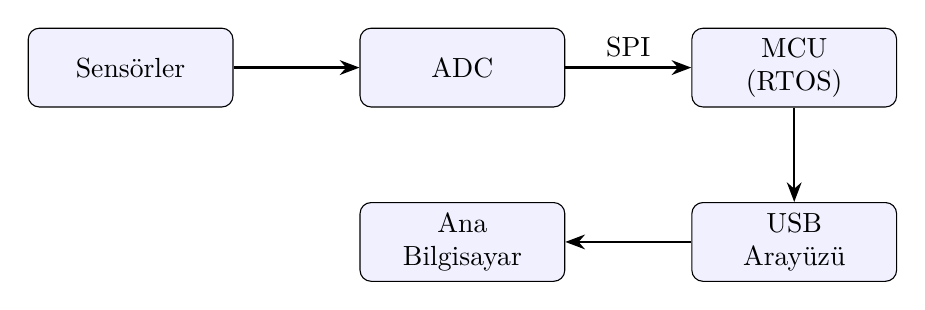
\begin{tikzpicture}[
    node distance=1.2cm and 1.6cm,
    block/.style={draw, rounded corners, minimum width=2.6cm, minimum height=1cm, align=center, fill=blue!6},
    arrow/.style={-{Stealth[length=2.5mm]}, thick}]
    \node[block] (sensor) {Sensörler};
    \node[block, right=of sensor] (adc) {ADC};
    \node[block, right=of adc] (mcu) {MCU\\(RTOS)};
    \node[block, below=of mcu] (usb) {USB\\Arayüzü};
    \node[block, left=of usb] (host) {Ana\\Bilgisayar};
    \draw[arrow] (sensor) -- (adc);
    \draw[arrow] (adc) -- node[above]{SPI} (mcu);
    \draw[arrow] (mcu) -- (usb);
    \draw[arrow] (usb) -- (host);
  \end{tikzpicture}
  \caption{Sistem mimarisi.}
  \label{fig:mimari}
\end{figure}

% !TEX root = ../main.tex
\section{Teknik Tasarım}
\label{sec:tasarim}

\subsection{Örnekleme}
Örnekleme periyodu $T_s$ ve kanal sayısı $C$ için toplam veri hızı
\cref{eq:veri-hizi} ile hesaplanır \parencite{knuth1984texbook}:
\begin{equation}
  R = \frac{C \cdot b}{T_s}
  \label{eq:veri-hizi}
\end{equation}
Burada $b$ örnek başına bit sayısıdır.

\subsection{Tasarım Kararları}
\begin{enumerate}[label=TK-\arabic*]
  \item Çift tamponlama ile DMA kullanılır.
  \item Zaman damgaları donanım sayacından alınır.
\end{enumerate}

% !TEX root = ../main.tex
\section{Gerçekleştirme}
\label{sec:gerceklestirme}

\Cref{lst:isr} örnekleme kesme rutinini gösterir.

\begin{lstlisting}[language=C, caption={ADC kesme rutini.}, label={lst:isr}]
/* ADC conversion-complete interrupt */
void ADC_IRQHandler(void)
{
    uint16_t sample = ADC1->DR;     /* read result */
    ring_buffer_push(&rb, sample);
    if (ring_buffer_full(&rb)) {
        notify_task(usb_task);
    }
}
\end{lstlisting}

% !TEX root = ../main.tex
\section{Test}
\label{sec:test}

\begin{table}[htbp]
  \centering
  \caption{Test durumları ve gereksinim izlenebilirliği.}
  \label{tab:testler}
  \begin{tabular}{@{}llll@{}}
    \toprule
    \textbf{Test} & \textbf{Gereksinim} & \textbf{Yöntem} & \textbf{Sonuç} \\
    \midrule
    TC-01         & \req{FR-01}         & Otomatik test   & Geçti          \\
    TC-02         & \req{FR-02}         & Otomatik test   & Geçti          \\
    TC-03         & \req{NFR-01}        & Güç ölçümü      & Geçti          \\
    TC-04         & \req{NFR-02}        & Kod incelemesi  & Beklemede      \\
    \bottomrule
  \end{tabular}
\end{table}

% !TEX root = ../main.tex
\section{Sonuçlar}
\label{sec:sonuclar}

Ölçülen ortalama güç tüketimi \qty{128.4}{\milli\watt} olup \req{NFR-01}
sınırının altındadır (\cref{tab:testler}). Ayrıntılı ölçümler
\cref{app:olcumler} içinde verilmiştir \parencite{lamport1994latex}.


\printbibliography[heading=bibintoc,title={Kaynaklar}]

\appendix
\crefalias{section}{appendix}
% !TEX root = ../main.tex
\section{Ölçüm Verileri}
\label{app:olcumler}

\begin{tabular}{@{}rS@{}}
  \toprule
  Ölçüm & {Güç (\si{\milli\watt})} \\
  \midrule
  1     & 127.9                    \\
  2     & 128.8                    \\
  \bottomrule
\end{tabular}


\end{document}
